\documentclass[12pt, a4paper,oneside]{report}
\usepackage[T1]{fontenc}
\usepackage[utf8]{inputenc}
\usepackage{braket}
\usepackage{geometry}
\geometry{a4paper,top=1.5cm, bottom=1.5cm}
\usepackage{titlesec}
\titleformat{\chapter}{\normalfont\huge}{\thechapter.}{20pt}{\huge\it}
\usepackage{newlfont}
\textwidth=450pt\oddsidemargin=0pt
\usepackage{amsthm}
\usepackage{amsmath}
\usepackage{amssymb}
\usepackage{graphicx}
\usepackage[english]{babel}
\usepackage{listings}
\usepackage{xcolor}
\usepackage{wrapfig}
\begin{document}
\begin{titlepage}
	\begin{center}
		{{\Large{\textsc{Liceo "I. Newton" di Chivasso}}}} \rule[0.1cm]{15.8cm}{0.1mm}
		\rule[0.5cm]{15.8cm}{0.6mm}
		{\small{\bf LICEO SCIENTIFICO\\
				Indirizzo scienze applicate}}
	\end{center}
	\vspace{15mm}
	\begin{center}
		\vspace{8cm}
		{\LARGE{\bf APPUNTI}}\\
		\vspace{19mm} {\large{\bf Corso di Matematica Olimpionica}}
	\end{center}
	\vspace{50mm}
	\par
	\noindent
	\begin{minipage}[t]{0.47\textwidth}
		{\large{\bf Davide PECCIOLI}}
	\end{minipage}
	\hfill
	\vspace{3cm}
	\begin{center}
		{\large{\bf $1^a$ e $2^a$ superiore }}
	\end{center}
\end{titlepage}
\chapter{Successioni}
	\section{Aritmetiche  $\to n_a=n_{a-1}+k$}
	\begin{itemize}
	\item punto di partenza$\to a_0$
	\item ragione $\Delta a=d$
	\end{itemize}
	\[
	\Set{a_0;a_0+d;a_0+2d; \dots}; a_n=a_{n-1}+d=a_0+nd
	\]
	\[
	\sum_{i=0}^n a_i=\frac{(n+1)(a_0+a_0+nd)}{2}
	\]
	\section{Geometriche $\to n_a=kn_{a-1}$}
	\begin{itemize}
		\item punto di partenza$\to a_0$
		\item ragione $\bigl(\frac{a_n}{a_{n-1}}\bigr)=q$
	\end{itemize}
	\[
	\Set{a_0;ka_0;k^{2}a_0; \dots}; a_n=ka_{n-1}=k^{n}a_0
	\]
	\[
	\sum_{i=0}^{n}a_i=a_0\frac{1-q^{n+1}}{1-q}
	\]
	\subsection{Serie}
	\textit{Successioni protratte all'infinito}
	\begin{itemize}
		\item $q\ge1\Rightarrow$
		\[
		S_\infty=\sum_{i=0}^{\infty}a_0\cdot q^i=+\infty
		\]
		\item $q<1\Rightarrow$
		\[
		q^2<q\Rightarrow\lim_{n \to \infty}q^{n+1}\to 0\Rightarrow
		\]
		\[
		\sum_{i=0}^{\infty}a_i=a_0\cdot\frac{1}{1-q}
		\]
	\end{itemize}
\chapter{Polinomi}
	\[
	p(x)=a_nx^n+a_{n-1}x^{n-1}+\dots+a_0
	\]
	Alcuni teoremi non dimostrati:
	\begin{enumerate}
		\item $p(x)=q(x)\Leftrightarrow a_{n_p}=a_{n_q}; a_{{n-1}_p}=a_{{n-1}_q}:\dots;a_{0_p}=a_{0_q} \forall a$
		\item Se due polinomi di grado $n$ hanno $n+1$ punti in comune allora saranno uguali
		\item $p(x) \land f(x) \Rightarrow p(x)=f(x)\cdot q+r$
		\item $p(x)=a_nx^n+a_{n-1}x^{n-1}+\dots+a_0\Rightarrow p(1)=\sum_{i=0}^{n}a_i$
		\item $p(x)=a_nx^n+a_{n-1}x^{n-1}+\dots+a_0\Rightarrow p(0)=a_0$
		\item $p(-1)$ è uguale alla differenza tra i coefficenti delle $x$ con esponente pari e di quelle con esponente dispari
		\[
		p(x)=a_nx^n+a_{n-1}x^{n-1}+\dots+a_0\land \{a_n=a_{2u}\lor a_n=a_{2u+1}\}\Rightarrow p(-1)=\sum_{i=0}^{u}a_{2i}-\sum_{i=0}^{u}a_{2i-1}
		\]
	\end{enumerate}
\chapter{Calcolo combinatorio}
\section{Permutazioni}
	\subsection{Semplici}
	Calcolare il numero di modi in cui si possono disporre $n$ elementi senza ripetizioni
	\[
	P_n=n!
	\]
	\newtheorem*{esempio}{Esempio}
	\begin{esempio}
		Quanti sono gli anagrammi della parola "case"?
		$4!=4\cdot3\cdot2=24 $
	\end{esempio}
	\subsection{Con Ripetizioni}
	Calcolare il numero di modi in cui si possono disporre $n$ elementi di cui $m$ ripetizioni
	\[
	P_n^m=\frac{n!}{m!}
	\]
	\begin{esempio}
		Quanti sono gli anagrammi della parola "cocomero"?\\
		\[
		\frac{8!}{3!\cdot2!}=\frac{8\cdot7\cdot6\cdot5\cdot4\cdot3\cdot2}{3\cdot2\cdot2}=\frac{40320}{12}=3360
		\]
	\end{esempio}
\section{Disposizioni}
	\subsection{Semplici}
	Calcolare il numero di modi in cui posso mettere $n$ oggetti in $k$ posti, senza ripetizioni, in cui l'odine è importante
	\[
	D_{n,k}=\frac{n!}{(n-k)!}
	\]
	\subsection{Con Ripetizioni}
	Calcolare il numero di modi in cui posso mettere $n$ oggetti in $k$ posti, con possibili ripetizioni, in cui l'odine è importante
	\[
	D'_{n,k}=n^k
	\]
\section{Combinazioni}
	\subsection{Semplici}
	Calcolare il numero di modi in cui si possono mettere $n$ oggetti in $k$ posti senza possibili ripetizioni, in cui l'ordine non è importante
	\begin{itemize}
		\item numero di sottoinsiemi fattibili con $k$ elementi presi da $n$ elementi totali
	\end{itemize}
	\[
	C=\binom{n}{k}=\frac{n!}{(n-k)!\cdot k!}
	\]
	\subsection{Con Ripetizioni}
	Calcolare il numero di modi in cui si possono mettere $n$ oggetti in $k$ posti con possibili ripetizioni, in cui l'ordine non è importante
	\[
	C=\binom{n+k-1}{k}=\binom{n+k-1}{n-1}
	\]
	\section{Coefficiente binomiale}
	\begin{itemize}
		\item {\LARGE$\binom{a+b}{a}=\binom{a+b}{b}$}
		\item {\LARGE$\binom{n}{0}=1$}
		\item {\LARGE$\binom{n}{n}=1$}
		\item {\LARGE$\sum_{i=0}^{n}\binom{n}{i}=2^n$}
	\end{itemize}
\chapter{Geometria}
	\newtheorem*{euclide1}{I Teorema di Euclide}
	\newtheorem*{euclide2}{II Teorema di Euclide}
	\newtheorem*{pitagora}{Teorema di Pitagora}
	\section{Triangoli}
	\subsection{Punti Particolari}
	\paragraph{Incentro}
	Il centro della circonferenza inscritta, \textit{incentro}, è l'intersezione delle bisetrici.
	\[
	p\to\text{semiperimetro}\qquad r\to\overline{IT}
	\]
	\[
	A_{A\hat{B}C}=r\cdot p
	\]
	\\
	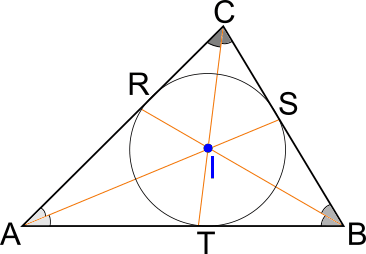
\includegraphics{In.jpg}
	\vspace{10cm}
	\paragraph{Circocentro}
	Il centro della circonferenza circoscritta, \textit{circocentro}, è il punto d'intersezione delle assi.
	\[
	R\to\text{raggio circonferenza circoscritta}\qquad\overline{AB}=a\qquad\overline{BC}=b\qquad\overline{AC}=c
	\]
	\[
	R=\frac{a\cdot b\cdot c}{4A_{A\hat{B}C}}
	\]
	\\
	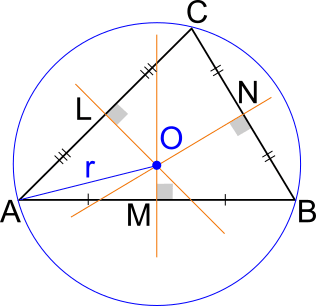
\includegraphics{Out.jpg}
	\paragraph{Baricentro}
	Il punto d'incontro delle mediane, il \textit{baricentro}, è sempre interno	
	\[
	\overline{AG}=2\overline{GN} \qquad \overline{BG}=2\overline{GL} \qquad \overline{CG}=2\overline{GM}
	\]
	\\
	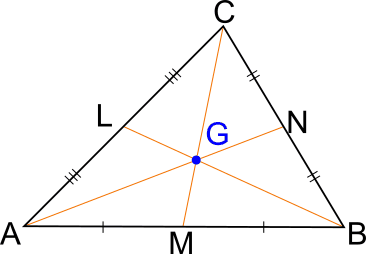
\includegraphics{Bar.jpg}
	\paragraph{Ortocentro}
	Il punto d'incontro delle altezze, l'\textit{ortocentro}\\
	\\
	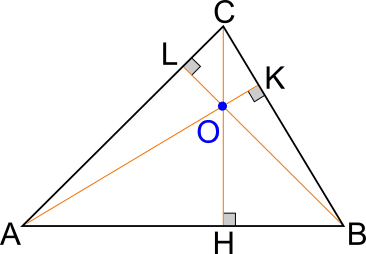
\includegraphics{Ort.jpg}
	\subsection{Teoremi}
	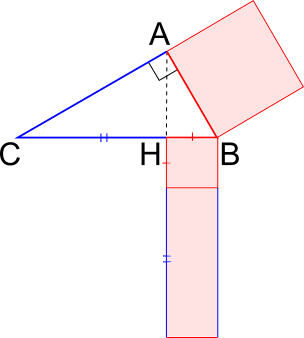
\includegraphics{Eu1.jpg}	
	\begin{euclide1}
	In un triangolo rettangolo il quadrato costruito su un cateto è equivalente al rettangolo avente come dimensioni l'ipotenusa e la proiezione del cateto stesso sull'ipotenusa
	\end{euclide1}
	\[
	\overline{AB}^2=\overline{CB} \cdot \overline{BH}\qquad\overline{HB}:\overline{AB}=\overline{AB}:\overline{CB}
	\]
	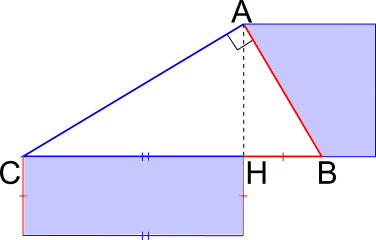
\includegraphics{Eu2.jpg}
	\begin{euclide2}
	In un triangolo rettangolo il quadrato costruito sull'altezza relativa all'ipotenusa è equivalente al rettangolo avente per dimensioni le proiezioni dei cateti sull'ipotenusa stesso
	\end{euclide2}
	\[
	\overline{AH}^2=\overline{BH}\cdot\overline{CH}
	\qquad
	\overline{CH}:\overline{AH}=\overline{AH}:\overline{BH}
	\]
	\\
	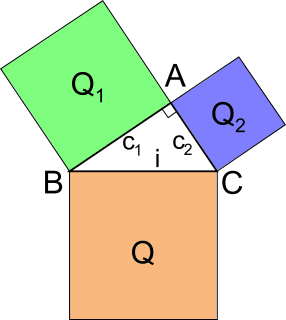
\includegraphics{Pit.jpg}
	\begin{pitagora}
	In un triangolo rettangolo il quadrato costruito sull'ipotenusa è equivalente alla somma dei quadrati costruiti sui cateti
	\end{pitagora}
	\[
	i^2=c^2_1+c^2_2
	\]
	\newpage
	\subsection{Formule}
	\vspace{1cm}
	\paragraph{Formula di Erone}
	Siano $a, b, c$ i lati di un triangolo, e $p$ il semiperimetro dello stesso. Sarà possibile trovare l'area ($A$) di questo triangolo utilizzando la sequente formula:
	\[
	A=\sqrt{p\cdot(p-a)\cdot(p-b)\cdot(p-c)}
	\]
	\vspace{1mm}
	\paragraph{Terne Pitagoriche}
	Considerando il Teorema di Pitagora: $a^2+b^2=c^2$, ecco le formule necessarie per calcolare le terne pitagoriche
	\[
	\underbrace{a=m;\qquad b= \frac{(m+1)(m-1)}{2};\qquad c=\frac{(m^2+1)}{2}}
	\]
	\[
	b; c\in\mathbb{N}\forall m|m=2q \land q \notin\mathbb{N}
	\]
	\vspace{3mm}
	\[
	\underbrace{a=2m;\qquad b=(m+1)(m-1);\qquad c=(m^2+1)}
	\]
	\[
	b; c\in\mathbb{N}\forall m|m=2q \land q \in\mathbb{N}
	\]
	\paragraph{Teorema di Stewart}
	Questo teorema è riassumibile dalla frase: "a \textbf{man} and his \textbf{dad} put a bomb (\textbf{bmb}) in the sink (\textbf{cnc})\\
	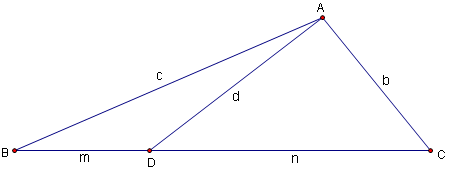
\includegraphics{Ste.jpg}\\
	\[
	man + dad = bmb + cnc
	\]
	\[
	man + ad^2 = mb^2 + nc^2
	\]
	\section{Circonferenza e cerchio}
	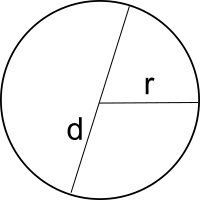
\includegraphics{Ci.jpg}
	\textbf{Formule}
	\[
	2p=2\pi r
	\]
	\[
	A=\pi r^2
	\]
	\subsection{Poligoni inscritti}
	Sia $n$ il numero di lati del poligoni inscritto in una circonferenza di raggio $r$, e $l_n$ la lunghezza del lato del poligono
	\[
	l_3=r\cdot\sqrt{3}\qquad l_4=r\cdot\sqrt{2}\qquad l_6=r
	\]
	\section{Goniometria}
		\subsection{Formule Goniometriche}
			\subsubsection{Sottrazione del coseno}
			\[cos(\alpha-\beta)\neq cos\alpha - cos\beta \]
			\begin{wrapfloat}{figure}{i}{0pt}
			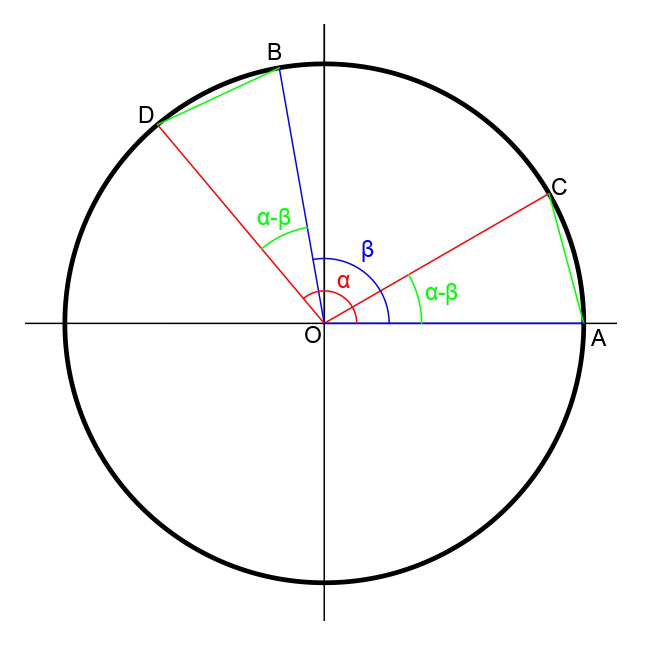
\includegraphics{SottCos.jpg}
			\end{wrapfloat}
\chapter{Teoria dei numeri}
	\section{Classi di resto}
	\begin{align*}
	a:b=q \text{ con resto }r\implies & b \text{ DIV }a=q \\
	a=b\cdot q+r \qquad\qquad\qquad & \colorbox{yellow}{b\text{ MOD }a=r}
	\end{align*}
	\colorbox{yellow}{$b\text{ MOD }a=r$} $\implies$ $[b]_a=[r]_a$ $\to$ Queste sono classi di resto.\\
	Per qualsiasi intero $n$ esistono $n-1$ classi di resto \textit{modulo} $n$\\
	\begin{align*}
	n=[0];\dots;[n-1] \qquad \text{\textbf{ESEMPIO: }} 7=[0];[1];\dots;[&6]\\
	[-&1]
	\end{align*}
	\paragraph{Operazioni con le classi di resto}
	\subparagraph{Somma, sottrazione e prodotto}
	Le prime tre operazioni base della matematica si comportano in maniera abbastanza prevedibile anche utilizzando le classi di resto; ecco qualche esempio.\\
	\textit{Stiamo lavorando \emph{modulo} 7}
	\begin{align*}
	&[1]+[4]=5\\
	&[6]+[6]=[12]=[5]\\
	&[3]-[1]=[2]\\
	&[1]\cdot[4]=[4]\\
	&[6]\cdot[6]=[36]=[1]\\
	&[-1]\cdot[-1]=[1]
	\end{align*}
	\subparagraph{Divisione}
	Osserviamo adesso come si comporta la divisione:
	\begin{align*}
	&[3]:[2]=[3]\cdot\colorbox{yellow}{$[2]^{-1}$}\\
	&\colorbox{yellow}{$[2]^{-1}$}=\colorbox{green}{$[x]$}\\
	&[2]\cdot\colorbox{green}{$[x]$}=[1]\implies x=4\\
	&[3]\cdot[4]=[12]=\colorbox{red}{$[5]$}
	\end{align*}
	\paragraph{Utilizzo delle classi di resto}
	\subparagraph{Semplificazione delle potenze}
	Ecco un semplice problema: con che cifra termina il numero $2007^{2010}$? 
	Dato che ci viene richiesta solo l'ultima cifra, possiamo considerare, anzichè $2007$, $[2007]_{10}=[7]$.\\
	Adesso consideriamo le potenze di [7]:
	\begin{align*}
	&[7]^1=[7]\\
	&[7]^2=[9]\\
	&[7]^3=[3]\\
	&[7]^4=[1]\\
	&[7]^5=[7]\\
	&[7]^6=[9]\\
	\end{align*}
	Possiamo immediatamente notare che esiste una certa ciclicità delle potenze.\\
	Diciamo quindi che 
	\[
	[7]^n=[7]^{[n]_4}
	\]
	Possiamo ora risolvere il problema iniziale: 
	\[[2007^{2010}]_{10}=[7]^{[2010]_4}=[7]^{[2]}=[9]\]
	\subparagraph{Criteri di divisibilità}
	Iniziamo con elencare i criteri di divisibilità più noti:
	\begin{itemize}
		\item Ogni intero modulo $2^n$ è uguale alle sue ultime $n$ cifre modulo $2^n$
		\item Ogni intero modulo $5^n$ è uguale alle due ultime $n$ cifre modulo $5^n$
		\item Ogni intero modulo 3 o 9 è uguale alla somma delle sue cifre modulo 3 o 9
		\item Ogni intero modulo 11 è uguale alla somma delle sue cifre di posizione dispari meno la somma delle cifre di posizione pari modulo 11
	\end{itemize}
	Adesso proviamo a dimostrare il criterio di congruenza \emph{modulo 3} utilizzando le classi di resto\\
	Sfruttiamo la scrittura polinomiale del numero:
	\[3457=7\cdot1+5\cdot10+4\cdot100+3\cdot1000\]
	\[[3457]_3=[7]_3+[5]_3\cdot[10]_3+[4]_3\cdot[100]_3+[3]\cdot[1000]_3\]
	\begin{align*}
	&[10^1]_3=[1]_3\\&[10^2]_3=[1]_3\\&[10^3]_3=[1]_3\\&\dots\\&[10^n]_3=[1]_3\\
	\end{align*}
	Possiamo quindi riscrivere il numero:
	\[[3457]_3=[7]_3+[5]_3+[4]_3+[3]_3\]
	\[[3457]_3=[7+5+4+3]_3=[3+4+5+7]_3=[1]_3\]
	Ecco quindi dimostrato il criterio di divisibilità \emph{modulo 3}
	\subparagraph{Residui quadratici}
	Data un'equazione con radici razionali in due incognite, prima di cercare di risolverla sarebbe meglio stabilire se ammette soluzioni:
	\[x^2+y^2=175\]
	Esiste un metodo molto veloce per stabilirlo: utilizzare i residui quadratici di 4
	\[
	\begin{cases}
	x\implies x^2\\
	[0]\implies[0]\\
	[1]\implies[1]\\
	[2]\implies[0]\\
	[3]\implies[1]\\
	\end{cases}
	\]
	Possiamo quindi stabilire che $x^2+y^2$ può assumere solamente certi valori\\ \emph{modulo 4}: $\{0;1;2\}$.\\
	Studiamo ora $[175]_4$: $[175]_4=[3]$, di conseguenza l'equazione riportata sopra è impossibile
		\section{Equazioni lineari diofantee}
	Le equazioni diofantee sono tutte quelle equazioni in due incognite a coefficienti razionali di cui si devono sapere le soluzioni intere.
	\[ax+by=c\]
	Perché queste equazioni possano avere soluzioni ci sono alcune condizioni:
	\[m.c.m.(a; b)|c\]
	\[a>b\]
	Mentre la prima condizione è fondamentale perchè esistano soluzioni, la seconda è una convenzione, utile per gli algoritmi di risoluzione
	\paragraph{Algoritmo di risoluzione}
	Per risolvere queste equazioni ci si può affidare all'algoritmo di Euclide, che prevede diversi passaggi:
	\begin{itemize}
		\item Trasformare l'equazione in modo tale che $c=1$
		\[ax+by=c\implies ax+by=1\]
		\item Sfruttare 
	\end{itemize}
\end{document}

